This application will take the wind tunnel data provided and scale it based on wind speed provided in this interface, and the building dimensions provided in the General Information. The theory on scaling wind tunnel data is provided in the theory. The data for the winnd tunnel is provided in a JSON file format. That file contains information on model dimensions, model wind speed, and model frequency, tap locations and time varying pressure tap coefficients.

\begin{figure}[!htbp]
  \centering {
    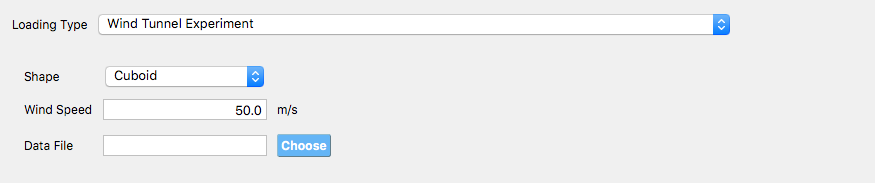
\includegraphics[width=0.8\textwidth]
    {usage/figures/windTunnelExperiment.png} }
  \caption{Wind Tunnel Experiment  Wind Loading Event}
  \label{fig:dedm_hrp}
\end{figure}

\begin{enumerate} 
\item The user to select the shape of the building, currently onlu Cuboid shapes are permitted.
\item The Wind Speed.
\item The file containing the experimental data.
\end{enumerate}

For this event, the wind speed can be a random variable.




